\section{Auswertung}
\label{sec:Auswertung}

\subsection{Bestimmung der Größe der Fehlstellen im Acrylblock}

Die Höhe $h$ des Acrylblocks beträgt $8,35\,\si{\centi\meter}$ 
und die Schallgeschwindigkeit in Acryl beträgt $c_A=2730\,\si{\meter\per\second}$\cite{kent2}.
Die gemessene Zeit des A-Scans ohne Fehlstelle beträgt $t=60,5\,\si{\micro\second}$.

In Tabelle 1 befinden sich die Schalllaufzeiten des A-Scans von der oberen $t_\text{A,o}$ 
und unteren $t_\text{A,u}$ Kante zur Fehlstelle sowie 
die damit und mithilfe der Gleichung 7 berechneten Abstände zur oberen $s_\text{A,o}$ und unteren
$s_\text{A,u}$ Kante, abzüglich der $0,2\,\si{\centi\meter}$ dicken Schutzschicht der Sonde, dessen
Verzögerung in jeden Scan einfließt. Aus den beiden Abständen 
lassen sich die Durchmesser der Fehlstellen 
\begin{align}
d_\text{A} = h_\text{A} - (s_\text{A,o} + s_\text{A,u})
\end{align}
berechnen, welche ebenfalls in Tabelle 1 aufgelistet sind.

\begin{table}[H]
  \centering
  \caption{Gemessene Abstände der Fehlstellen in dem Acrylblock.}
  \begin{tabular}{c c c c c c}
    \toprule
  Fehlstelle & $t_o/\symup{\mu}$s & $t_u/\symup{\mu}$s & $s_\text{A,o}/$cm & $s_\text{A,u}/$cm & $d_\text{A}$cm\\
    \midrule
    3  & 46,7 &  11,9  & 5,33 & 1,21  & 1,71  \\
    4  & 41,4 &  18    & 4,71 & 1,93  & 1,62  \\
    5  & 36   &  24,1  & 4,07 & 2,66  & 1,53  \\
    6  & 30,5 &  30,5  & 3,41 & 3,41  & 1,43  \\
    7  & 24,5 &  36,3  & 2,70 & 4,10  & 1,45  \\
    8  & 18,9 &  42,1  & 2,04 & 4,79  & 1,43  \\
    9  & 13,1 &  47,9  & 1,35 & 5,48  & 1,43  \\
    10 & 7,5  &  53,7  & 0,69 & 6,16  & 1,40  \\
    11 & 42,5 &  13,3  & 4,84 & 1,38  & 2,04  \\
    \bottomrule
  \end{tabular}
\end{table}

\subsection{Untersuchung des Auflösungsvermögens}
In Abbildung 3 bis 5 ist der A-Scan mit Sonden unterschiedlicher Frequenz
von der oberen Kante zu den Fehlstellen 1 und 2 dargestellt, an dessen Positionen
sich die Cursor befinden.

\begin{figure}[H]
  \centering
  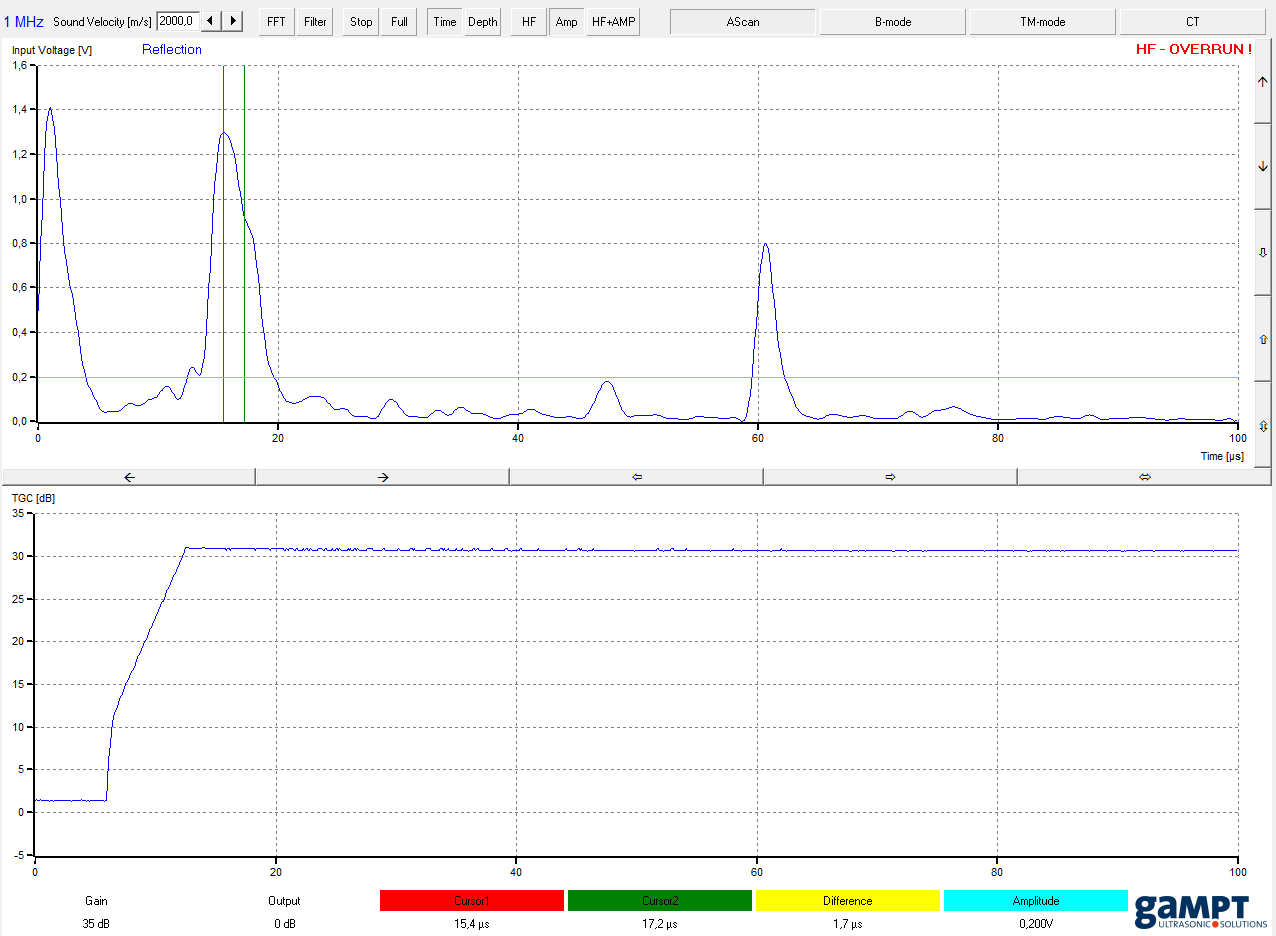
\includegraphics[height=7cm]{1mhz.png}
  \caption{Untersuchung der Löcher 1 und 2 mit Sonde mit 1MHz.}
  \label{fig:1mhz}
\end{figure}

\begin{figure}[H]
  \centering
  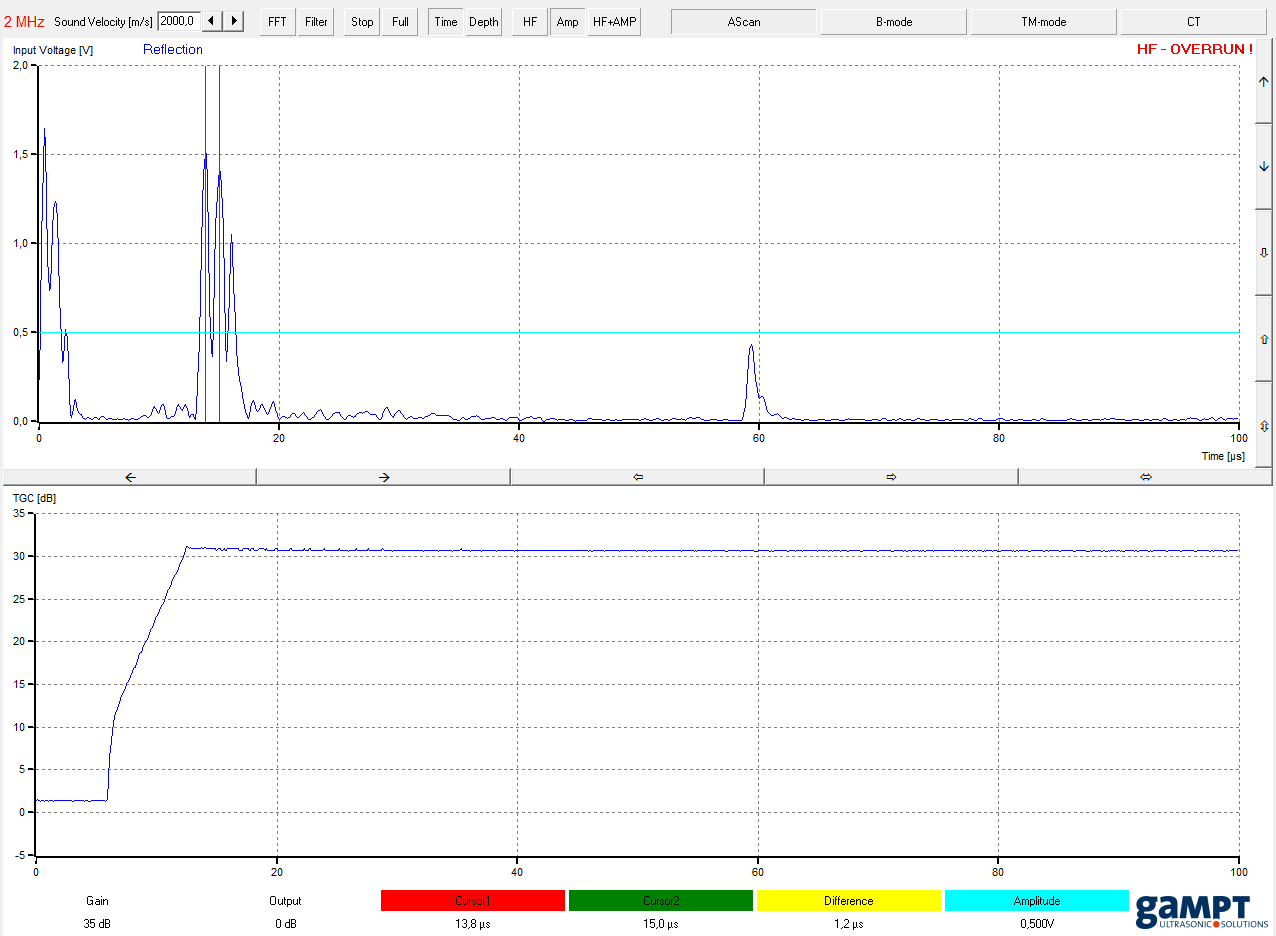
\includegraphics[height=7cm]{2mhz.png}
  \caption{Untersuchung der Löcher 1 und 2 mit Sonde mit 2MHz.}
  \label{fig:2mhz}
\end{figure}

\begin{figure}[H]
  \centering
  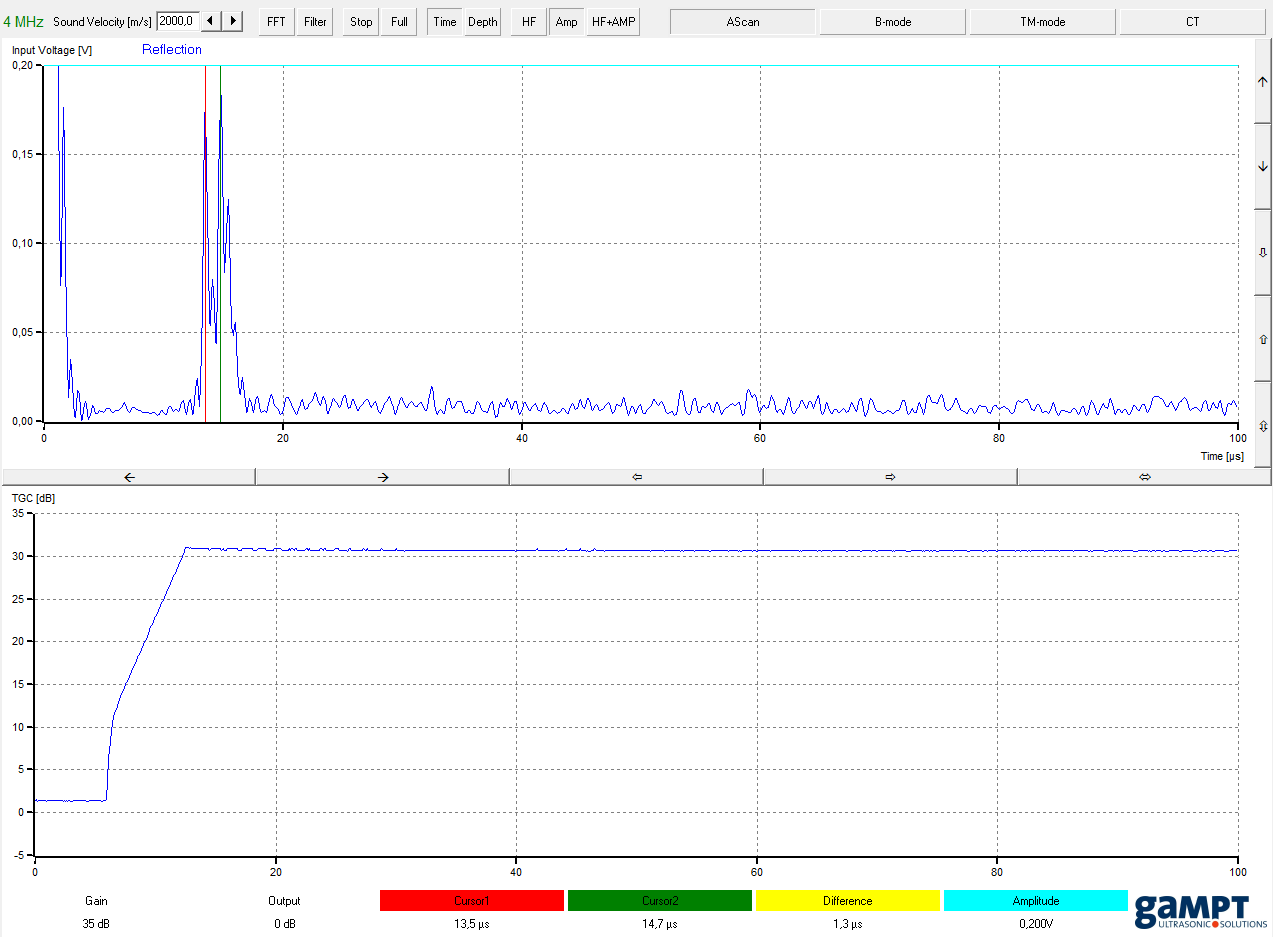
\includegraphics[height=7cm]{4mhz.png}
  \caption{Untersuchung der Löcher 1 und 2 mit Sonde mit 4MHz.}
  \label{fig:4mhz}
\end{figure}


\subsection{Bestimmung der Abmessungen der Störstellen mittels B-Scan}
In Abbildung 6 und 7 ist der B-Scan des Blocks dargestellt. Mit der Eingabe der Schallgeschwindigkeit in Acryl
$c_\text{A}$ in das verwendete Programm lassen sich die Abstände zur oberen $s_\text{B,o}$ und
unteren $s_\text{B,u}$ Kante auslesen. Aus diesen lässt sich
mit Gleichung 8 erneut der Durchmesser der Fehlstellen $d_\text{B}$ bestimmen. Die genannten Abstände und die
Durchmesser sind in Tabelle 2 notiert.

\begin{figure}[H]
  \centering
  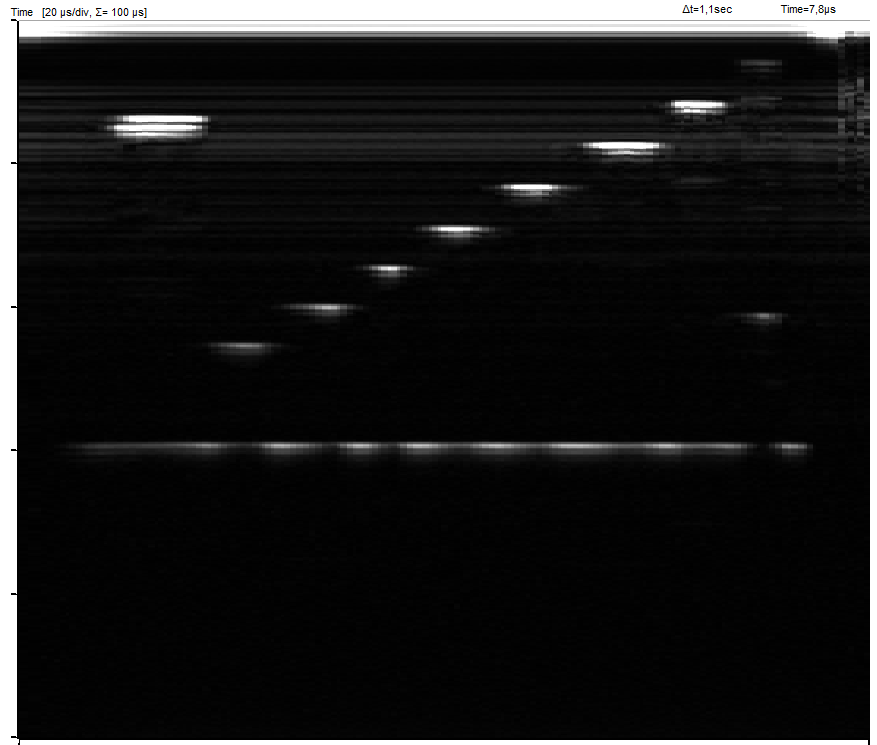
\includegraphics[height=7cm]{b-time-1.png}
  \caption{Abbildung des B-Scans von der oberen Kante.}
  \label{fig:acryl}
\end{figure}

\begin{figure}[H]
  \centering
  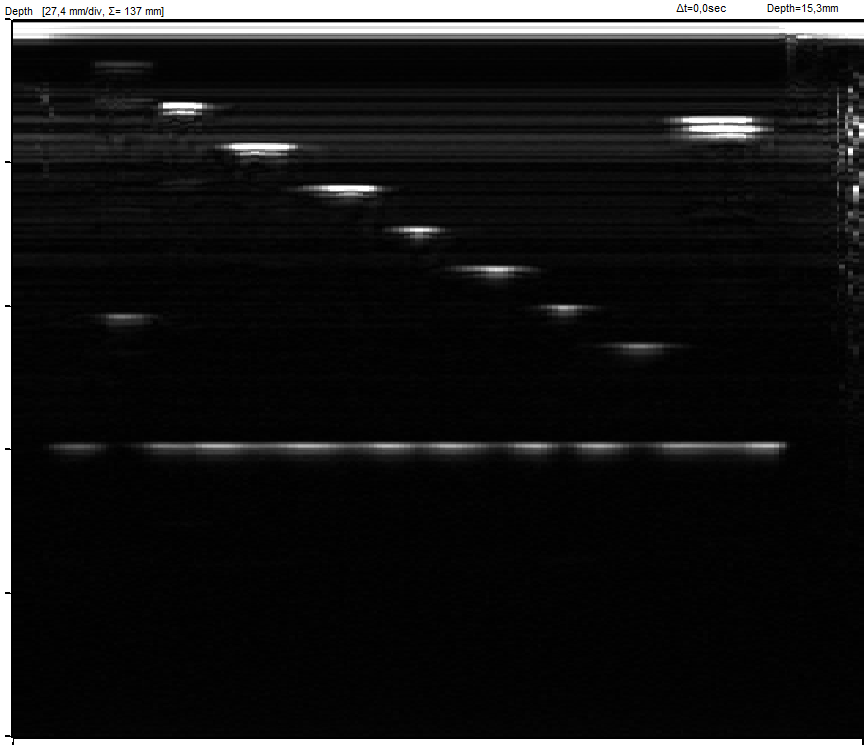
\includegraphics[height=7cm]{b-time-2.PNG}
  \caption{Abbildung des B-Scans von der unteren Kante.}
  \label{fig:acryl}
\end{figure}

\begin{table}[H]
  \centering
  \caption{Mittels B-Scan berechneten Abstände und Durchmesser.}
  \begin{tabular}{c c c c}
    \toprule
  Fehlstelle & $s_\text{B,o}/$cm & $s_\text{B,u}/$cm & $d_\text{B}/$cm\\
    \midrule
    3   & 6,24 & 1,49  & 1,02   \\
    4   & 5,5  & 2,33  & 0,92   \\
    5   & 4,77 & 3,15  & 0,83   \\
    6   & 4,03 & 4,03  & 0,69   \\
    7   & 3,22 & 4,83  & 0,7    \\
    8   & 2,42 & 5,61  & 0,72   \\
    9   & 1,64 & 6,41  & 0,7  \\
    \bottomrule
  \end{tabular}
\end{table}




\subsection{Bestimmung des Herzvolumens}
In Tabelle \ref{tab:1} werden für die 7 simulierten Herzschläge jeweils die gemessenen Amplituden $t_s$ und die daraus berechneten
Volumina $V_s$ aufgeführt. In Abbildung \ref{fig:TM} ist das Diagramm des erstellten TM-Scans zu erkennen, aus dem die besagten Amplituden
bestimmt werden. Das Luftvolumen, welches das Wasser beim Pumpen durch die bewegliche Membran verdrängt, wird als
Kugelsegment\cite{kent3} angenähert und ergibt sich zu
\begin{equation}
  V_s = \frac{h\pi}{6}\cdot(3r^2 + h^2),
\end{equation}
mit $h$ nach Gleichung 7.
Der Radius beträgt $r = 2,5 \: \symup{cm}$ und die Frequenz des simulierten
Herzschlags beträgt $f = 0,45\,\si{\hertz}$.

\begin{figure}[H]
  \centering
  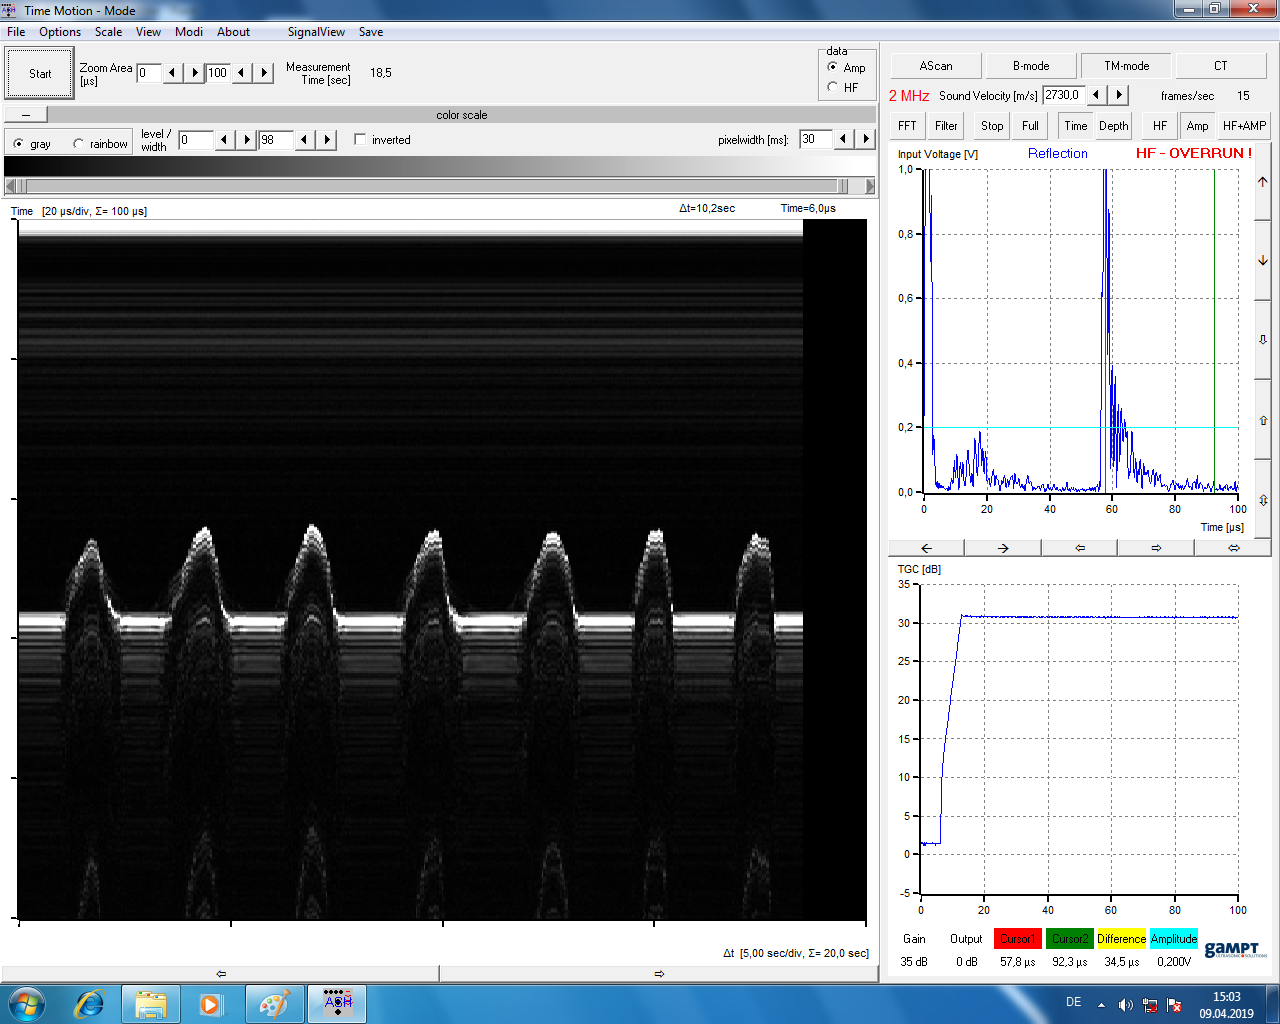
\includegraphics[height=7cm]{tm-herz.png}
  \caption{Abbildung des TM-Scans für den simulierten Herzschlag.}
  \label{fig:TM}
\end{figure}

\begin{table}[H]
  \centering
  \caption{Gemessene Amplituden bei Herzschlagsimulation.}
  \label{tab:1}
  \begin{tabular}{c c c }
    \toprule
  Schlag & $t_s/\symup{\mu s}$ & $V_s/\symup{cm^3}$ \\
    \midrule
    1  &  10,98 & 16,48     \\
    2  &  12,72 & 19,79     \\
    3  &  13,29 & 20,94     \\
    4  &  12,14 & 18,65     \\
    5  &  12,42 & 19,20     \\
    6  &  12,79 & 19,93     \\
    7  &  11,56 & 17,55     \\
    \bottomrule
  \end{tabular}
\end{table}

\noindent Als Mittelwert ergibt sich mittels Mittelwerts- und Standardabweichungsformel
 ein Volumen von $V_{m} = (18,93 \pm 1,41) \: \symup{cm^3}$.

\noindent Mithilfe der Gleichung zur Bestimmung des Herzvolumens\cite[S.5]{kent}
\begin{equation*}
  V_{Herz} = V_m \cdot f
\end{equation*}
ergibt sich das gesuchte Herzvolumen zu
\begin{equation*}
  V_{Herz} = (8,5 \pm 0,6) \: \symup{\frac{cm^3}{s}}.
\end{equation*}
%\vspace*{20mm}